%--------------------------------------------------------------------------a---
\chapter{\babTiga}
%-----------------------------------------------------------------------------%

Bab ini menjelaskan tentang metode penelitian yang digunakan beserta langkah-langkahnya.

Berdasarkan latar belakang masalah, rumusan masalah, tujuan penelitian, dan ruang lingkup pengerjaan yang telah dibahas pada bab satu, metodologi penelitian yang digunakan dalam penelitian ini adalah sebagai berikut.

\section{Studi Literatur}
Pada tahap ini dilakukan studi literatur tentang teori-teori dan metode yang mendukung penelitian ini. Studi literatur yang dilakukan adalah mempelajari tentang Voronoi Diagram dan implementasinya, mempelajari lebih dalam tentang Weighted Voronoi Diagram dan research tentangnya, \textit{tools} dan aplikasi yang dapat digunakan untuk mengimplementasikan Weighted Voronoi Diagram, macam-macam \textit{distance}, \textit{hotspot} dan Wi-Fi, serta mempelajari tentang \textit{hotspot} di Universitas Indonesia.

\subsection{Diagram Voronoi yang Digunakan}
Setelah melakukan riset terhadap jenis diagram Voronoi yang ada, ditentukan bahwa diagram Voronoi yang digunakan dalam penelitian ini adalah \textit{weighted Voronoi diagram}. Hal ini dikarenakan \textit{todo alasan} 

\subsection{Distance yang Digunakan}
Setelah melakukan riset mengenai jenis \textit{distance} yang digunakan dalam penelitian ini, ditentukan bahwa \textit{distance} yang digunakan adalah Euclidean \textit{distance}. Hal ini dikarenakan jarak Euclidean merupakan jenis jarak yang paling sederhana.

\subsection{Pemetaan Weighted Voronoi Diagram dan Hotspot}
Dalam penelitian ini, \textit{weight} dalam \textit{weighted Voronoi diagram} digambarkan dengan kekuatan sinyal dan bandwidth dari hotspot.

\section{Research Tools}
Untuk menggambarkan Weighted Voronoi Diagram diperlukan suatu \textit{tools} atau aplikasi. Terdapat berbagai macam \textit{tools} yang dapat digunakan untuk menggambarkan Weighted Voronoi Diagram. Setiap \textit{tools} yang ada memiliki fungsi dan penggunaannya masing-masing. Berikut merupakan hasil riset untuk \textit{tools} yang telah dilakukan.

\begin{table}[H]
\centering
\caption{Hasil Riset \textit{Tools}}
\label{research-tools}
\scalebox{0.7}{%
\begin{tabular}{|l|c|c|c|}
\hline
 & \multicolumn{1}{l|}{Menghitung Diagram Voronoi} & \multicolumn{1}{l|}{Menggambar Diagram Voronoi} & \multicolumn{1}{l|}{Menggambar Peta} \\ \hline
R Studio & v & v & v \\ \hline
Open Voronoi & v &  &  \\ \hline
Power Voronoi Diagram & v &  &  \\ \hline
ArcGIS &  & v & v \\ \hline
\end{tabular}}
\end{table}

Setelah melakukan riset untuk \textit{tools} yang akan digunakan dalam penelitian ini, ditentukan bahwa \textit{tools} yang akan digunakan adalah RStudio. RStudio dipilih karena selain dapat melakukan perhitungan diagram voronoi, dalam RStudio juga bisa melakukan \textit{plotting} untuk diagram dengan \textit{output} berupa gambar .png.

\section{Data}
Untuk melakukan penelitian ini diperlukan informasi tentang lokasi dari \textit{access point} \textit{hotspot} yang ada di Universitas Indonesia. Untuk mendapatkan informasi tersebut perlu menghubungi Direktorat Sistem & Teknologi Informasi (DSTI) Universitas Indonesia. DSTI merupakan lembaga yang bertanggung jawab untuk mengelola sarana dan prasarana yang berhubungan dengan Teknologi Informasi di Universitas Indonesia. 

Data yang digunakan dalam penelitian ini adalah data lokasi dari \textit{access point} yang ada di Universitas Indonesia. Data yang didapat dari DSTI {\ui} masih berupa data mentah. Data tersebut harus diolah dulu untuk bisa digunakan dalam penelitian ini.

\section{Implementasi Dasar}
Implementasi dasar yang akan dilakukan adalah memetakan data yang didapat dari DSTI ke dalam peta {\ui}. Setiap satu lokasi \textit{access point} digambarkan sebagai satu titik dalam peta. Penempatan dari setiap titik sesuai dengan koordinat yang telah didapat dari pengolahan data.

\section{Penambahan Bobot dan Jangkauan}
Masing-masing titik diberikan bobotnya sebagai bobot dari Weighted Voronoi Diagram. Bobot ini sesuai dengan beban dan bandwidth dari setiap \textit{access point}. Selain bobot juga ditambahkan jangkauan dari setiap \textit{access point} yang berupa lingkaran-lingkaran yang berpusat pada titik tersebut. Berdasarkan titik dan bobotnya, kemudian digambarkan diagram voronoi untuk setiap titik.

\section{Modifikasi Implementasi dan Data}
Dalam peta, titik merupakan gambaran dari lokasi \textit{access point}. Lingkaran merupakan gambaran dari jangkauan suatu \textit{access point}. Bobot dari suatu titik merupakan penggambaran dari beban kapasitas yang harus di-\textit{cover} oleh satu \textit{access point}. Diagram Voronoi berperan sebagai penggambaran dari lokasi yang harus dijangkau oleh suatu \textit{access point}. 

Kondisi ideal adalah kondisi dimana setiap daerah dalam peta berada di dalam lingkaran. Yang berarti setiap daerah mendapatkan sinyal \textit{hotspot}. Kondisi inilah yang akan dicapai dalam penelitian ini. 

\begin{figure}
	\centering
	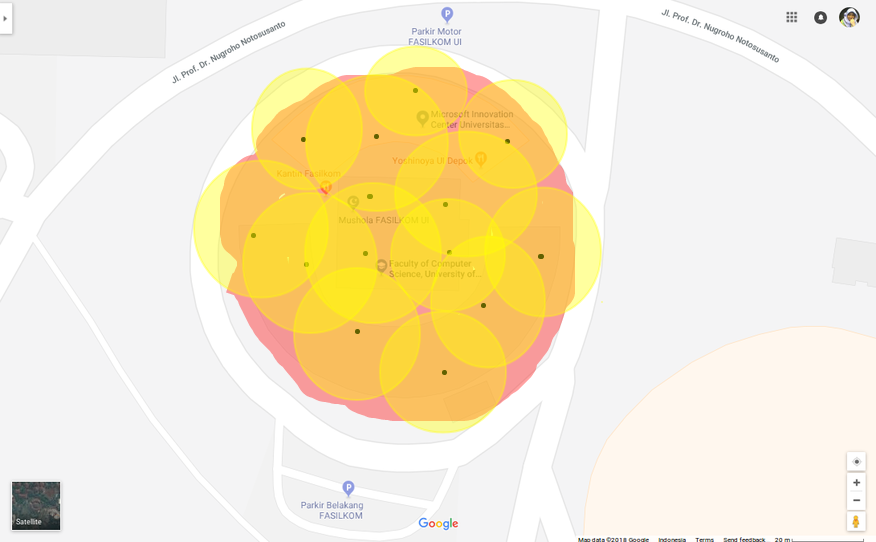
\includegraphics[width=10cm]{pics/fasilkom-demand-coverage.png}
	\caption{Kondisi Ideal}
	\label{fig:kondisiIdeal}
\end{figure}

Kondisi yang tidak ideal adalah kondisi di mana terdapat daerah dalam peta yang tidak berada di dalam lingkaran. Hal ini berarti daerah tersebut tidak mendapatkan sinyal Wi-Fi. Untuk itu perlu ditambahkan satu titik baru di daerah di luar lingkaran sehingga daerah tersebut mendapatkan sinyal Wi-Fi. 

\begin{figure}
	\centering
	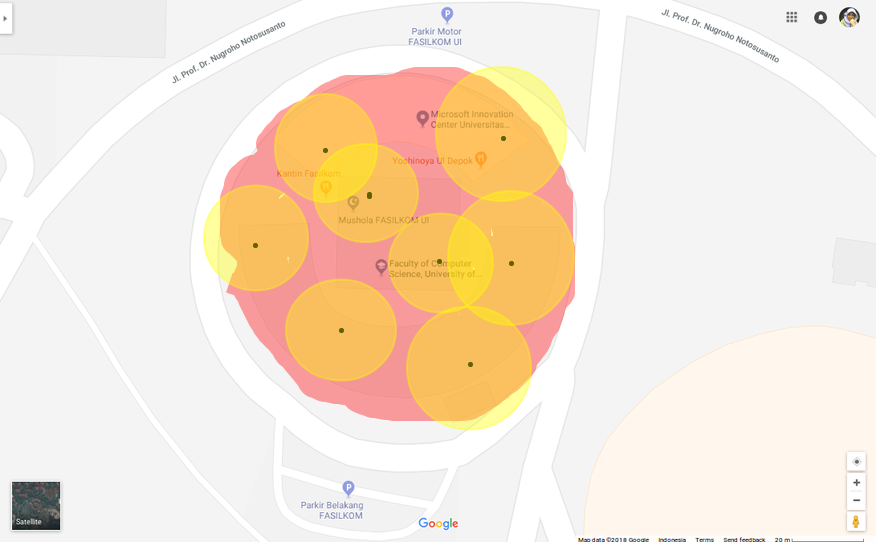
\includegraphics[width=10cm]{pics/fasilkom-demand-coverage-minus.png}
	\caption{Kondisi Tidak Ideal}
	\label{fig:kondisiTidakIdeal}
\end{figure}

Proses penambahan titik ini dilakukan secara iteratif sehingga setiap daerah berada dalam jangkauan sinyal Wi-Fi atau berada di dalam lingkaran.

\begin{figure}
	\centering
	\includegraphics[width=14cm]{pics/tahapanPenelitian.png}
	\caption{Tahapan Penelitian}
	\label{fig:tahapanPenelitian}
\end{figure}

\section{Pemetaan dari Paper}

n max = jumlah maksimal station baru = jumlah maksimal \textit{hotspot} device

n min = jumlah minimal station baru = jumlah minimal \textit{hotspot} device

n = jumlah station baru = jumlah \textit{hotspot} device baru

sigma W = total active load =

sigma P = total active power kapasitas ekonomi = 

Se max = nilai maksimum dari kapasitas ekonomi (kapasitas x rasio load) =

Se min = kapasitas ekonomi minimum dari tipe kandidat dari substation
eta = relaxation faktor = 

M = jumlah grup dari skema kombinasi kapasitas =  

m = same with M? =

k = jumlah tipe kandidat substation = jumlah tipe kandidat \textit{hotspot} device

CZi = cost investasi dari i tipe kandidat transformer substation = 

CUi = cost operasi tahunan dari i tipe kandidat dari transformer 

substation =

r0 = diskon rate = 

ms = periode depresiasi dari substation = 

xi = jumlah dari i tipe kandidat konstruksi transformer = 

Si = kapasitas dari i tipe kandidat substation (load rate sudah di 

peretimbangkan) =

Sgxist = kapasitas existing station (load rate sudah dipertimbangkan) = 

W = total load = 

cos phi = power factor = 

\section{\textit{Distance} yang Digunakan}
Dalam penelitian ini menggunakan Euclidean \textit{distance} karena Euclidean merupakan \textit{distance} yang paling sederhana. 

\section{Evaluasi keberhasilan}
Parameter keberhasilan dalam penelitian ini ada dua, yaitu menggambarkan Weighted Voronoi Diagram dari lokasi-lokasi \textit{access point} di {\ui} beserta jangkauannya dan mendapatkan lokasi-lokasi \textit{access point} baru sehingga setiap daerah mendapatkan sinyal Wi-Fi.

%\section{Desain dan Implementasi}
%\subsection{Desain Sistem}

%Desain dari sistem yang akan dibuat adalah sebagai berikut:

%\begin{enumerate}
%\item Pemetaan lokasi hotspot

%Lokasi hotspot saat ini dipetakan ke dalam peta 

%\item Penggambaran diagram voronoi

%Digambarkan weighted voronoi diagram dari persebaran hotspot saat ini, dengan kekuatan signal dari hotspot sebagai weight.

%\item Dilakukan pengecekan untuk setiap perbatasan dua atau lebih diagram. Pengecekan yang dilakukan adalah kekuatan signal dan bandwidth (terdapat threshold minimalnya)

%\item Kalau kurang dari threshold maka perlu ditambah device baru di titik tersebut
%\item Berarti satu iterasi itu meliputi setiap dua atau lebih diagram.  Maksudnya dia akan mencari di setiap perbatasan mana saja yg kurang kapasitasnya.
%\item Setelah diketahui titik-titiknya, kemudian digambarkan device baru di titik-titik tersebut. (pemetaan lokasi hotspot baru)
%\item Setelah itu kembali ke tahap penggambaran diagram voronoi, dan seterusnya sampai tujuan tercapai (tidak ada titik yg di bawah threshold signal dan bandwidth minimal)
%\end{enumerate}

%\begin{figure}
%	\centering
%	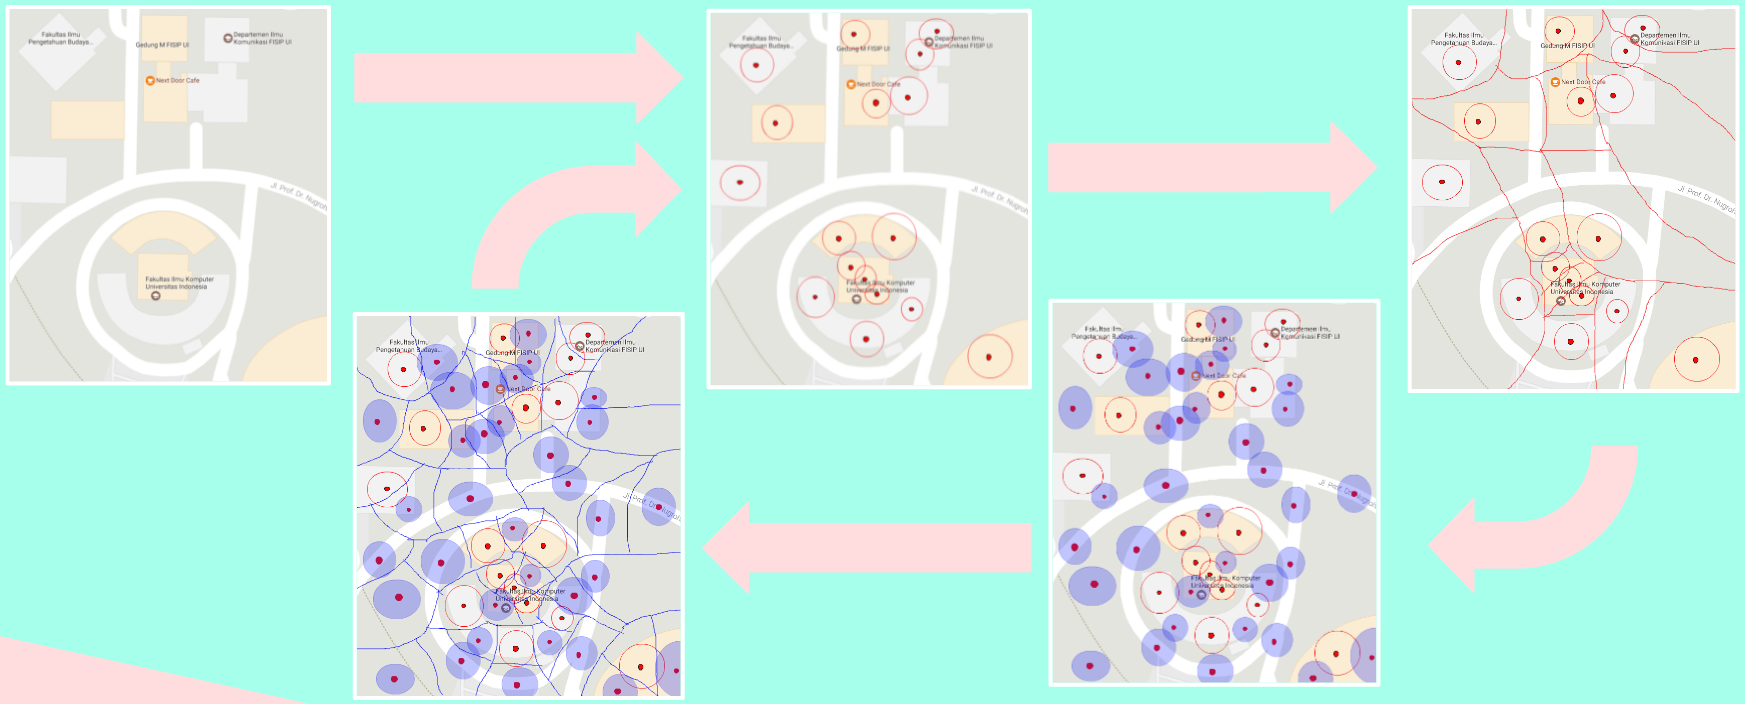
\includegraphics[width=14cm]{pics/desainProses.png}
%	\caption{Desain Proses}
%	\label{fig:desainProses}
%\end{figure}

%\subsection{Desain Interaksi}

%Desain interaksi dari sistem yang akan dibuat adalah sebagai berikut:

%\begin{enumerate}
%	\item User memasukkan peta, jumlah titik (hotspot) dan koordinat dari masing-masing titik.
%	\item Ditampilkan hasil pemetaan titik-titik hotspot ke dalam peta.
%	\item Digambarkan weighted voronoi diagram dari kumpulan titik-titik tersebut.
%	\item Dilakukan penghitungan kekuatan signal dan bandwidth untuk setiap perbatasan diagram.
%	\item Menampilkan lokasi dari calon hotspot baru.
%\end{enumerate}



%%-----------------------------------------------------------------------------%
%\section{Studi Literatur}
%-----------------------------------------------------------------------------%
%

%
%%-----------------------------------------------------------------------------%
%\section{Desain dan Implementasi}
%-----------------------------------------------------------------------------%
%
%Pada tahap ini akan dilakukan perancangan sistem yang akan dibuat, serta tahapan implementasi dari sistem tersebut.
%
%\subsection{Pemetaan Lokasi}
%
%Pada tahap ini akan dilakukan pemetaan lokasi-lokasi dari fasilitas umum yang akan dianalisis. Pemetaan akan dilakukan dengan menggunakan R Software, yaitu RStudio. Dalam peta yang dibuat terdapat informasi tentang lokasi-lokasi dari fasilitas umum yang akan dianalisis. Data tersebut digambarkan dalam format vektor, yaitu dalam bentuk \textit{area} untuk peta dari daerah yang akan dianalisis, serta bentuk \textit{point} untuk lokasi-lokasi dari fasilitas umum. %perlu tambah teori tentang RStudio?
%
%\subsection{Penggambaran Diagram Voronoi}
%
%Pada tahap ini akan dilakukan penggambaran diagram Voronoi pada peta yang telah dipetakan lokasi-lokasi fasilitas umum yang akan dianalisis. Penggambaran diagram Voronoi dilakukan dengan menggunakan Wolfram Alpha. Koordinat dari lokasi-lokasi pada peta di dalam tahap sebelumnya masing-masing  dipetakan ke Wolfram Alpha dan dibuat diagram Voronoi-nya menggunakan perintah VoronoiDiagram yang terdapat dalam paket ComputationalGeometry.  %teori tentang wolfram juga?
%
%Diagram Voronoi yang dihasilkan dari Wolfram Alpha kemudian dipetakan kembali ke dalam peta pada R Software. Hal ini dilakukan agar ruang lingkup atau daerah cakupan dari masing-masing lokasi fasilitas umum bisa terlihat dengan jelas.
%
%%Okay disini kalimat-kalimat kasarnya dulu. Jadi tuh desainnya apa ya? desain programnya? Kan aku mau bikin sesuatu yang bisa digunakan untuk mencari lokasi optimal untuk fasilitas umum. Nyari lokasinya pake apa? Pertama kan udah ada info tentang lokasi-lokasi fasilitas umum itu (udah ada peta yang isinya lokasi-lokasi fasilitas umum). Terus digambarlah diagram Voronoi di peta itu, jadi tau cakupan dari masing-masing fasilitas umum itu. 
%
%\subsection{Penambahan Data Spasial}
%
%Pada tahap ini akan dilakukan penambahan informasi-informasi yang terkait dengan data spasial untuk daerah dalam peta. Informasi-informasi yang ditambahkan diantaranya:
%
%\begin{itemize}
%\item[-] Data kepadatan penduduk di daerah tersebut
%\item[-] Tingkat permintaan akan fasilitas umum pada daerah tersebut
%\end{itemize}
%
%Informasi tersebut kemudian dipetakan ke dalam peta pada R Software dengan format vektor dalam bentuk \textit{area} dengan warna tertentu yang berbeda dengan warna peta dasar dan berbeda untuk masing-masing informasi. 
%
%Untuk tingkat kepadatan penduduk yang lebih tinggi akan dibuat dengan warna yang lebih pekat. Begitu juga untuk tingkat permintaan akan fasilitas umum pada daerah tersebut.
%
%%Kemudian mencari data untuk:
%
%- Kapasitas masing-masing fasilitas umum
%- Kepadatan penduduk di daerah tersebut
%- Demand untuk fasilitas umum tersebut di daerah itu
%
%\subsection{Perhitungan Kebutuhan Fasilitas Umum}
%
%Pada tahap ini akan dilakukan perhitungan jumlah kebutuhan fasilitas umum untuk suatu daerah dalam satu waktu. Perhitungan dilakukan dengan cara mengalikan jumlah penduduk dengan tingkat permintaan untuk fasilitas umum yang akan dianalisis. Hasil tersebut kemudian dibandingkan dengan kapasitas masing-masing fasilitas umum sehingga dapat diketahui apakah fasilitas umum tersebut bisa mencukupi kebutuhan di lingkungan tersebut.
%
%Tingkat kebutuhan akan fasilitas umum yang dinamis, membuat analisis mengenai lokasi yang optimal dari fasilitas umum ini perlu dilakukan sesuai dengan perubahan penduduk dan tingkat kebutuhan akan fasilitas umum tersebut.
%
%%Setelah mendapatkan data untuk daerah tersebut, kemudian bisa dihitung dengan kapasitas sekian, jumlah penduduk kali demand untuk daerah itu berapa, maka tempat itu cukup ga untuk melayani permintaan? Mungkin ga sekedar permintaan di satu waktu ya, karna untuk setiap waktu kan pasti jumlah permintaannya beda-beda.
%
%%Kalo rumah sakit contohnya, mungkin bisa dicari masa-masa orang sakit tuh kapan aja. Misalnya pas musim pancaroba, atau pas musim hujan. 
%
%%Tapi kan informasi tentang rate itu pasti per daerah ya, kaya misal perkabupaten atau perkecamatan. Sedangkan cakupan dari diagram Voronoi itu random, ga berbatas kecamatan atau kabupaten. Jadi harus ngitung dulu rata-rata dari tempat itu. Kaya misal satu daerah Voronoi itu gabungan dari 3 kecamatan, kan brarti ada porsi untuk masing2 kecamatannya seberapa luas. Jumlah penduduk dibagian itu berapa. Terus dicari rata2nya. Nah rata2 ini ga serta merta dibagi tiga, tapi harus disesuaikan sama bobotnya. Bobot luas dan jumlah penduduknya. 
%
%%Oke, udah tau kan semuanya brarti tinggal diitunglah cukup engganya. Kalo misal ga cukup atau berlebihan brarti ada yang harus diperbaiki. (Urusan memperbaiki ini kayanya di luar thesis ya? Eh tapi kan perlu tau lokasi optimalnya.) Oke brarti next nya cari lokasi optimal.
%
%\subsection{Penentuan Lokasi Baru}
%
%Pada tahap ini akan dilakukan pencarian titik lokasi baru untuk fasilitas umum di suatu daerah yang membutuhkan fasilitas umum tambahan. Penentuan lokasi dilakukan dengan menambahkan satu titik lokasi fasilitas umum pada peta dengan warna yang paling pekat. Hal ini dikarenakan daerah dengan warna paling pekat memiliki tingkat kebutuhan akan fasilitas umum lebih tinggi dibandingkan dengan daerah lainnya.
%
%%Pake apa? Kalo terlalu ringan (bersisa) mungkin ga masalah, tapi kalo kurang baru mungkin perlu ditambah. Nah tadi habis ditambah data kepadatan penduduk, demand, dll, jadi mapnya warnanya berubah sesuai dengan constraint2 tadi. Misal yg butuh banget fasilitas itu warnanya jadi merah tua. Nah, buat tau lokasi barunya mungkin bisa taruh aja tuh titik lokasi baru di daerah yg merah tua (pekat) itu. 
%
%\subsection{Rekomendasi Perubahan Lokasi}
%
%Pada tahap ini akan dicari lokasi optimal untuk fasilitas umum yang baru. Setelah peta dasar ditambahkan dengan fasilitas-fasilitas umum yang baru, peta tersebut akan diberikan perlakuan yang sama seperti pada tahap pertama hingga tahap terakhir. Pencarian lokasi baru ini dilakukan secara iteratif sehingga setiap daerah terpenuhi kebutuhan fasilitas umumnya.
%
%%Mungkin next nya setelah ditaruh lokasi baru itu jadi bisa diitung lagi optimalitas lokasi2 itu secara keseluruhan lagi. Terus, terus, sampe ketemu map yg paling optimal banget.
%
%%-----------------------------------------------------------------------------%
%\section{Evaluasi}
%-----------------------------------------------------------------------------%
%
%Pada tahap ini akan dilakukan percobaan terhadap sistem yang telah dibuat, untuk memastikan bahwa sistem tersebut telah berjalan sesuai rancangan. Setelah sistem berjalan dengan baik, maka akan dilanjutkan dengan evaluasi untuk sistem tersebut. Evaluasi dilakukan dengan berbagai macam input dan data, serta berbagai macam \textit{use case}.
